\documentclass{article}
\usepackage{fullpage,proof,url,amssymb,amsmath,graphicx}


\newtheorem{theorem}{Theorem}
 
\def\barp{\bar{p}}
\def\HHB{{\mathrm{HHB}}}
\def\CS{\mathrm{CS}}
\def\calX{\mathcal{X}}
\def\bbR{\mathbb{R}}
\def\dx{\mathrm{d}x}
%\def\HH{\mathrm{HH}}
%\def\lhs{\mathrm{lhs}}
%\def\rhs{\mathrm{rhs}}
%\def\dx{\mathrm{d}x}
%\def\dy{\mathrm{d}y}
%\def\dt{\mathrm{d}t}
%\def\bbR{\mathbb{R}}
\newenvironment{proof}{\paragraph{Proof:}}{\hfill$\square$}
 
\newtheorem{fact}{Fact}
\newtheorem{lemma}{Lemma}
\newtheorem{definition}{Definition}

\begin{document}

\title{Bregman spheres: Thales' theorem}

%\author{Frank Nielsen}
\date{\today}
\maketitle

% IG2016 p143  
\cite{IG-2016}

space of Bregman spheres \cite{BVD-2010}

% p64 

\begin{lemma}[Corollary 3.11~\cite{Amari-2007}, Problem 11.6~\cite{IG-2014}]
Consider a sphere $S=\{q : D(c:q)=r\}$ of center $c$ and radius $r$.
Then the $\nabla$-geodesic passing through $c$ intersects the sphere orthogonally.
The tangent autoparallel manifolds are $\nabla^*$-hyperplane.
\end{lemma}

\begin{proof}
...
\end{proof}


Recall Thales' theorem in Euclidean geometry
\begin{theorem}[Thales' theorem]
The triangle circumscribed to a circle with one side being a diameter is right-angle.
\end{theorem}

\begin{proof}
...
\end{proof}

This theorem is not to be confused with Thales' intercept theorem (basic proportionality theorem).
There are many proofs of Thales's (circle) theorem (e.g., using the sum of angles in a triangle to be $\pi$, using Pythagoras' theorem).


In a dually flat space, there are $2^3=8$ geodesic triangles\footnote{And $2^n$ types of geodesic $n$-gons.} ($6$ pseudo-triangles and $2$ dually flat triangles) passing through three vertices $p, q$ and $r$, depending on whether we choose the primal or dual geodesic for linking ay two of those points.
In general a dually flat space is not conformal but flat: The angles of (pseudo)-triangle (which triangle type?, purely primal or dual) sum up to $\pi$ and there exists a Pythagoras' theorem.
 
Let $(ab)$ denote the primal geodesic segment passing through $a$ and $b$, and $(ab)^*$ the dual geodesic segment. 

\begin{theorem}[Thales' Bregman theorem]
The triangle $(pq)^*(qr)^*$ circumscribed to a $\nabla$-circle with the  side $(pr)$ being a diameter is right-angle at $q$.
\end{theorem}

Note that $(pr)$ intersects the $\nabla$-circle orthogonally.

\begin{figure}%
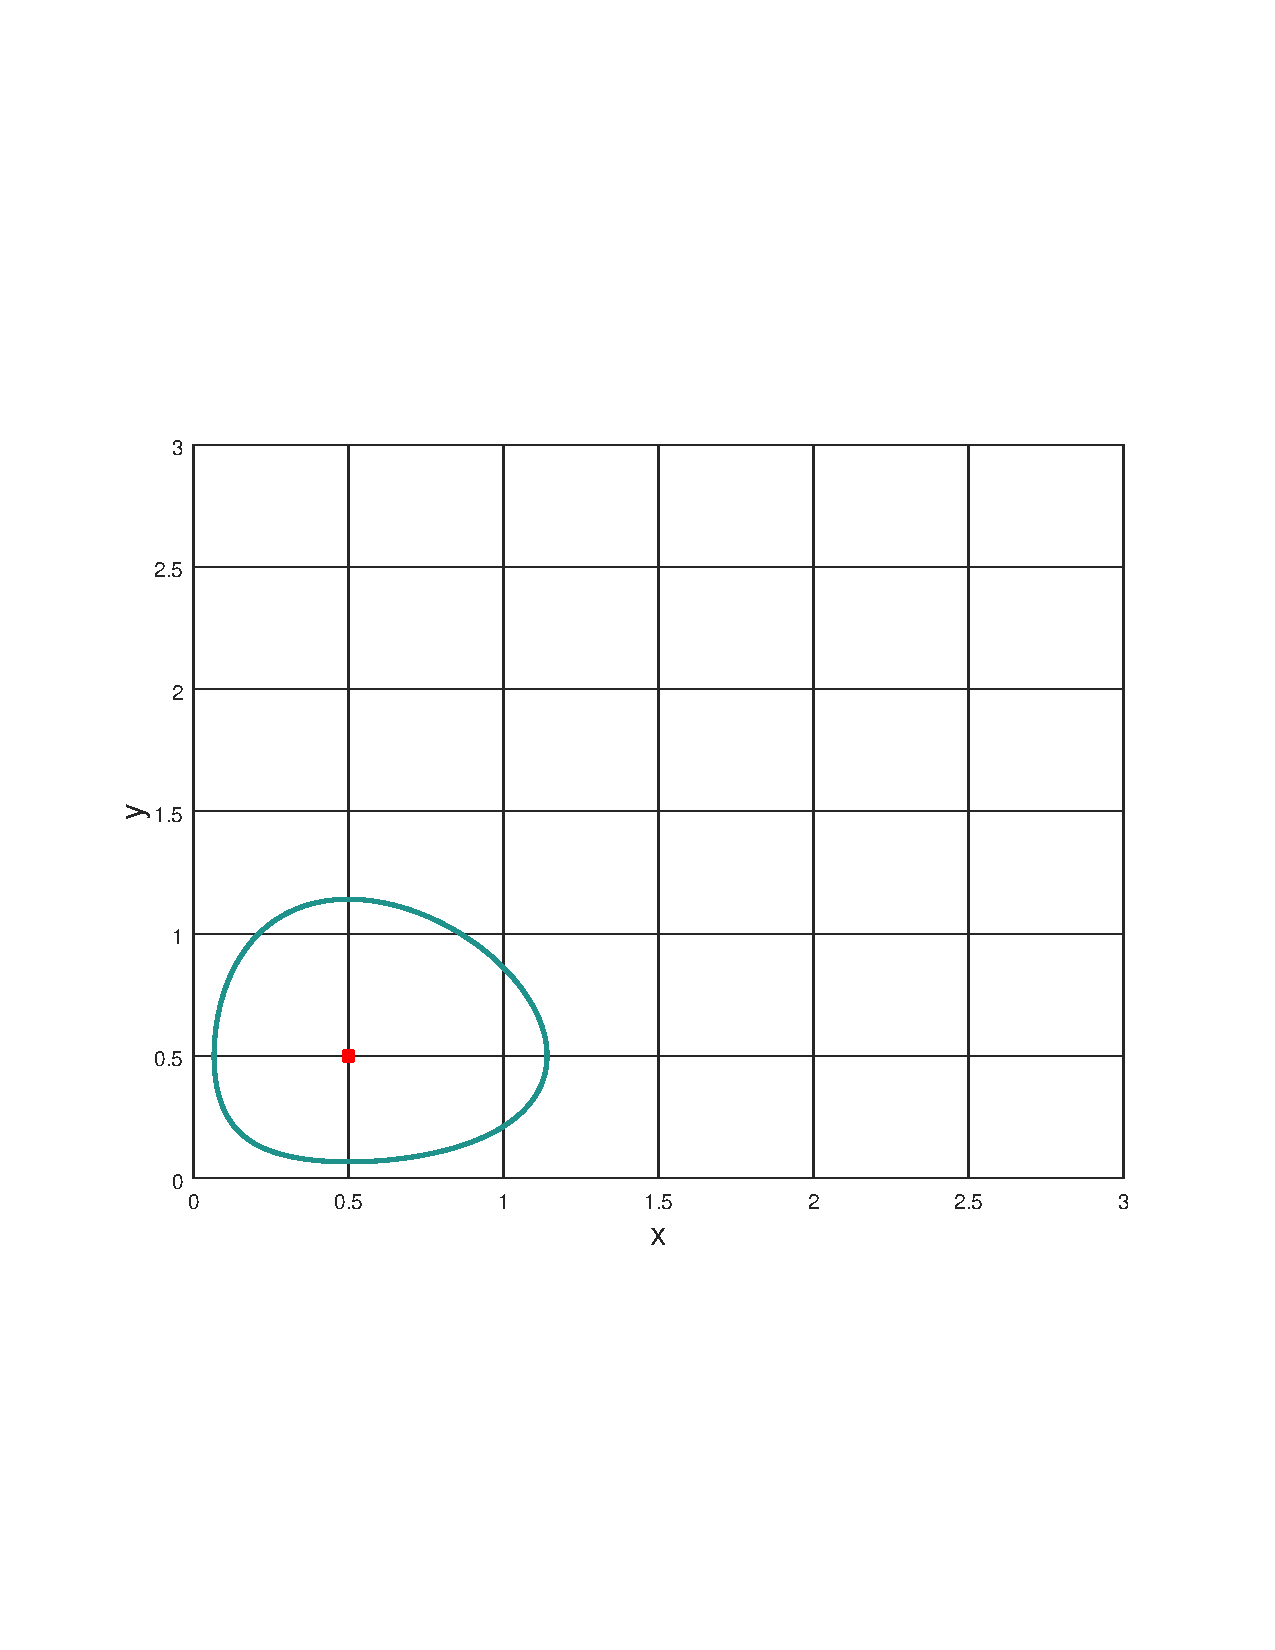
\includegraphics[width=0.8\columnwidth]{eKL-ball.pdf}%
\caption{An extended Kullback-Leibler ball of center $(\frac{1}{2},\frac{1}{2})$ and radius $\frac{3}{10}$ (defined on positive measures).}%
\label{}%
\end{figure}

% http://www.nabla.hr/Z_MemoHU-023.htm
Using space of spheres
Intersection of two planes: a line. That line intersecting the potential function and projecting back yields the intersection point of the sphere with a sphere.

\bibliographystyle{plain}
\bibliography{BregmanSphereBib}
\end{document}